\cleardoublepage

\section{IOS-Analyse
\label{section:iosanalysis}}
Apple verwendet MAC-Adress-Randomisierung seit der IOS Version 8, 
welche am 17. September 2014 veröffentlicht wurde.
Die Einführung von Randomisierung wurde nich nur als Absicht aufgefasst,
die Privatsphäre der Apple-Benutzer besser zu schützen. 
Es wurde spekuliert, dass Apple die eigene Positionierungstechnologie
IBeacon vorantreiben möchte, ein Service, der es erlaubt, IOS-Geräte 
zu lokalisieren und Pushnachrichten oder personalisierte Werbung auf diesen 
Geräten zu schalten.

In den folgenden Untersektionen werden die verschiedenen IOS-Versionen ab der
Version 8 analysiert und aufgezeigt, wie sich die Verschleierung von 
MAC-Adressen weiterentwickelt hat.
Es gilt noch zu erwähnen, dass Apple keine Dokumentationen für diese Features
herausgibt und sämtliche Informationen über verschiedene Quellen zusammengesucht 
werden müssen.
Eine Auflistung der Versionsgeschichte findet sich in der 
Tabelle~\ref{table:iosversionhistory}.

\subsection{Versionsgeschichte}
\begin{table}[H]
    \begin{tabularx}{\linewidth}{XXX}
        \toprule 
        \textbf{Aktuellste Version} & \textbf{Erscheinungsdatum} & \textbf{Letzte Version für} \\
        \midrule
        3.1.3 & 02.02.2010 & IPhone 2G \\
        4.2.1 & 22.11.2010 & IPhone 3G \\
        5.1.1 & 07.05.2012 & - \\
        6.1.6 & 21.02.2014 & IPhone 3GS \\
        7.1.2 & 30.06.2014 & IPhone 4 \\
        \rowcolor{lightgray}
        8.4.1 & 13.08.2015 & - \\
        \rowcolor{lightgray}
        9.3.5 & 25.08.2016 & - \\
        \rowcolor{lightgray}
        9.3.6 & 22.07.2019 & IPhone 4S \\
        \rowcolor{lightgray}
        10.3.3 & 19.07.2017 & IPhone 5C \\
        \rowcolor{lightgray}
        10.3.4 & 22.07.2019 & IPhone 5 \\
        \rowcolor{lightgray}
        12.4.7 & 20.05.2020 & IPhone 5S, IPhone 6 \\
        \rowcolor{lightgray}
        13.7 & 01.09.2020 & - \\
        \rowcolor{lightgray}
        14 & 16.09.2020 & - \\
        \bottomrule 
    \end{tabularx}
    \caption{Versionsgeschichte des iOS für iPhones, 
    alle grau eingefärbten Zeilen benutzen MAC Randomisierung
    \label{table:iosversionhistory}}
\end{table}

\subsection{iOS 8}
Das iOS 8 wurde am 2. Juni 2014 vorgestellt, am 14. September 2014
eingeführt und von den Geräten IPhone 4 bis 6 verwendet. 
Die Version 8 ist die erste, die bei IPhones bei Probe-Requests die 
MAC-Adresse randomisiert.
Die offizielle Ankündigung auf der Apple-Webseite ist in der 
Abbildung~\ref{figure:MACRandAnnoucement} ersichtlich.

\begin{figure}[h!]
    \centering
    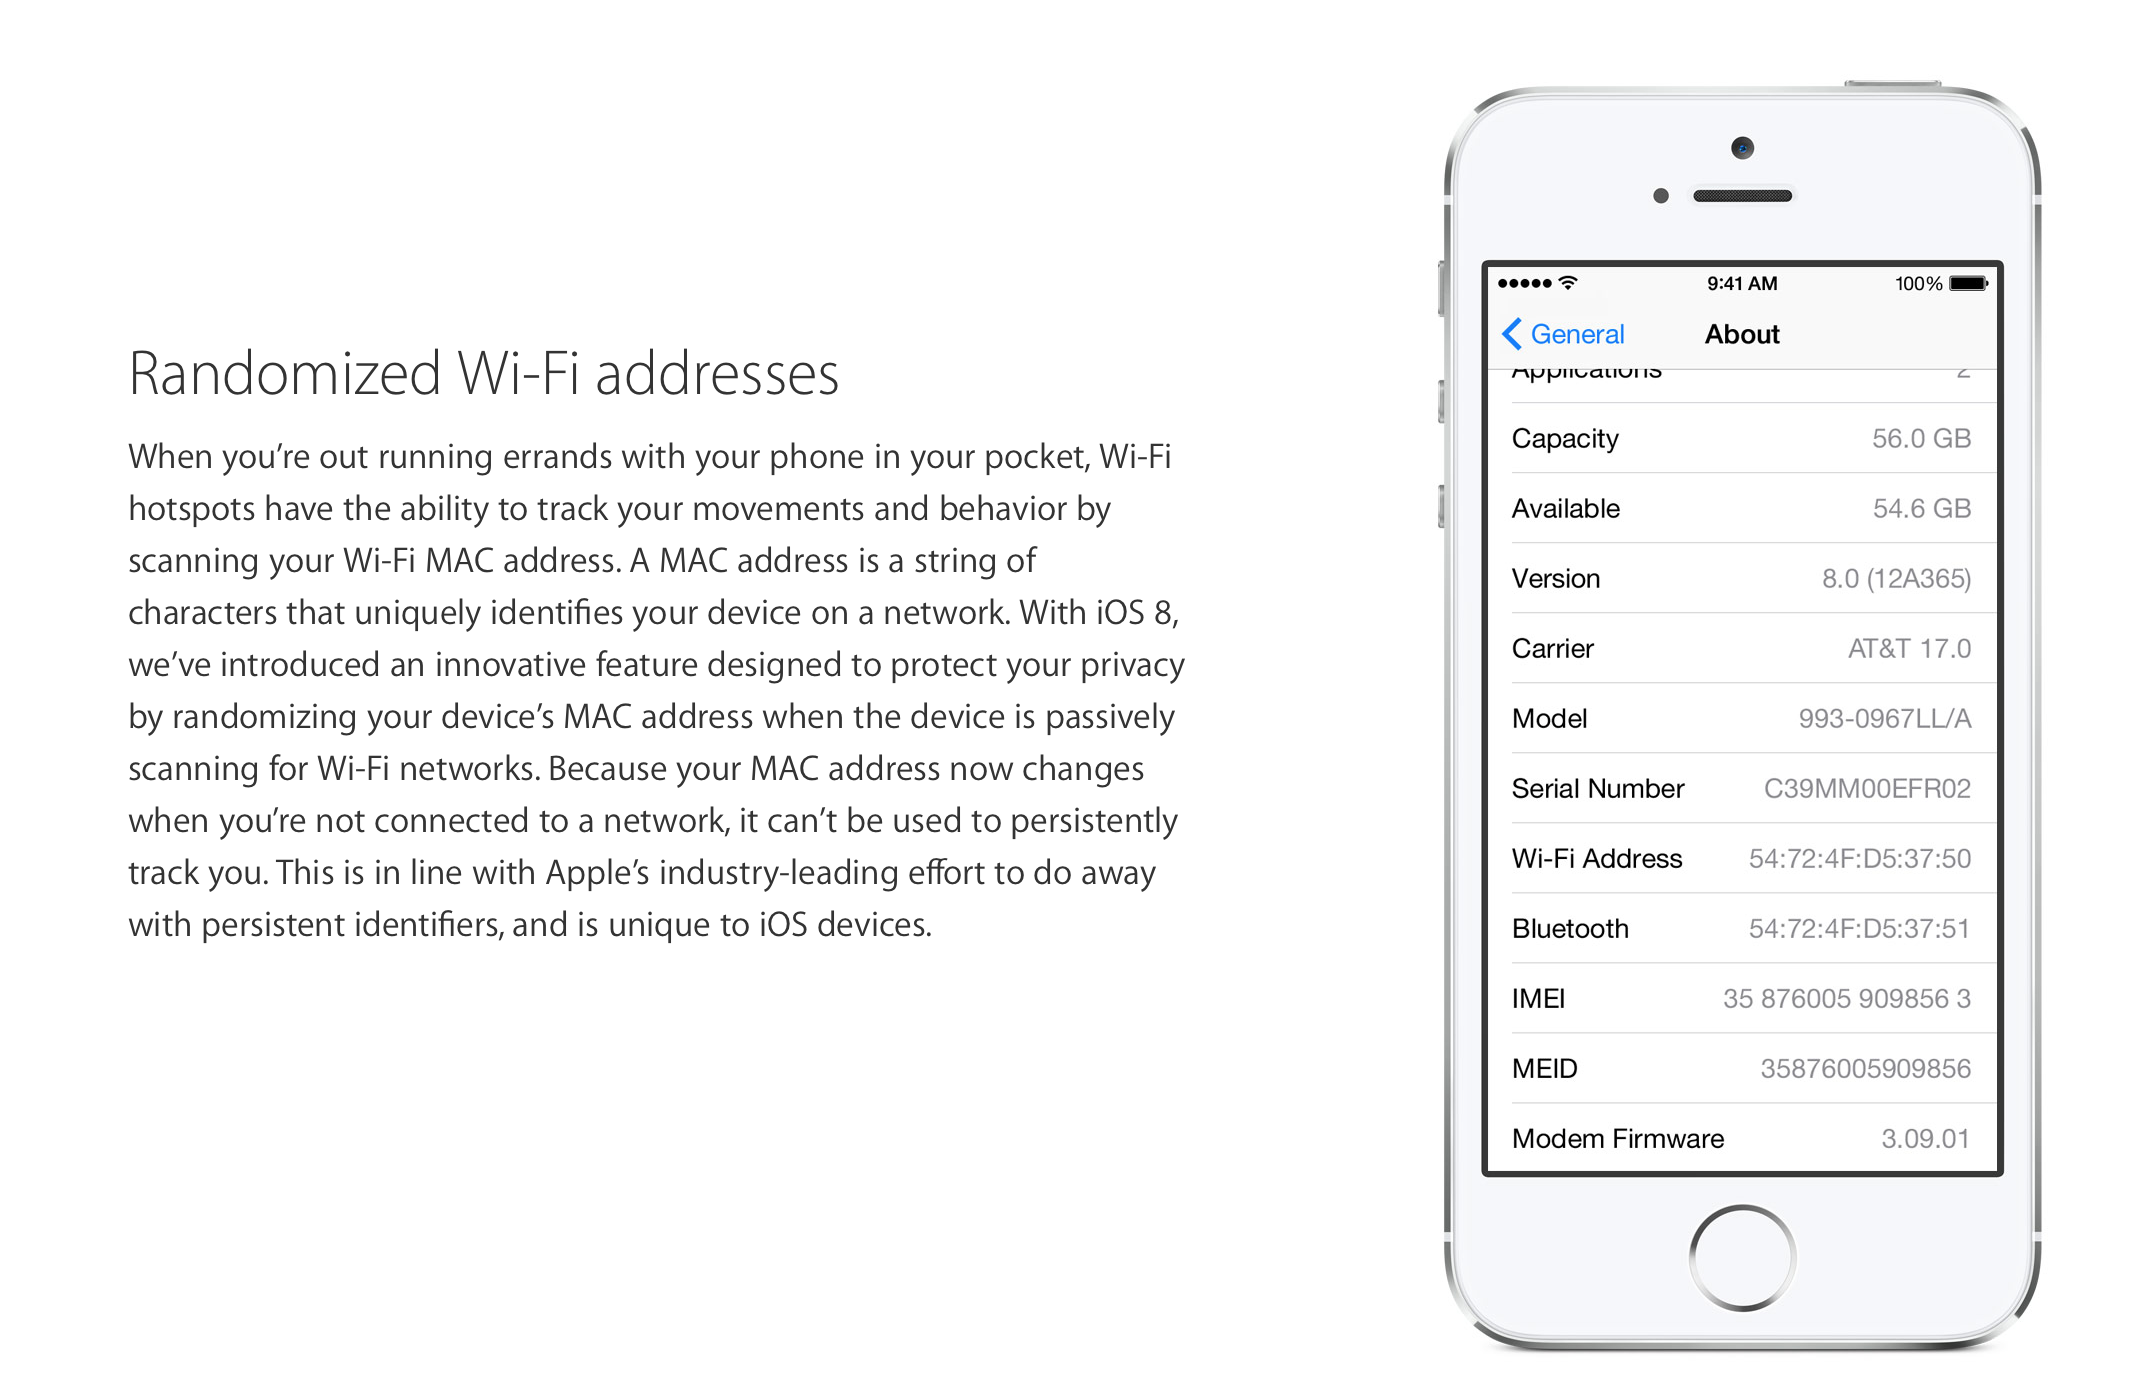
\includegraphics[width=1\linewidth]{Analyse/iOS8_rand_announcement.png}
    \caption{Offizielle Randomisierungs-Ankündigung von Apple}
    \label{figure:MACRandAnnoucement}
\end{figure}

Allerdings wird die Randomisierung nur dann ausgeführt, wenn die folgenden
drei Bedingungen erfüllt sind.

\begin{itemize}
    \item Das Wifi muss aktiviert sein, das Gerät darf aber nicht mit einem Hotspot assoziert sein.
    \item Das Smartphone muss sich im Sleep Mode befinden.
    \item Der Location Service muss in den privacy Settings explizit ausgeschaltet sein.
\end{itemize}

\clearpage

Somit wird die Randomisierung nur dann verwendet, wenn der Benutzer sich nicht
bereits mit einem Netzwerk verbunden hat, das Gerät gerade nicht verwendet und
explizit die Location Services ausgeschaltet hat.
Viele Applikationen diese Location Services aber voraus und 
die meisten Nutzer machen sich nicht den Aufwand, jedes Mal die Einstellungen
anzupassen, wenn sie eine Applikation verwenden wollen. 
Diese Faktoren haben dazu geführt, dass iOS-Geräte die MAC-Adresse häufig nicht 
zufallsgeneriert haben, obwohl Hard- und Software dies ermöglicht hätten.

\subsection{iOS 9}
Nachdem die Implementation der Randomisierung in der iOS Version 8 kritisiert
wurde, wurde das Verfahren in der Version 9 überarbeitet und verbessert.
In der Tabelle~\ref{table:iosversionninediff} ist der direkte Vergleich 
von iOS 8 zu iOS 9 ersichtlich.

\begin{table}[H]
    \begin{tabularx}{\linewidth}{|X|r|r|}
        \hline
            & \textbf{iOS 8} & \textbf{iOS 9} \\
        \hline
        Unassociated PNO Scans & Yes & Yes \\
        Unassociated ePNO Scans & Yes & Yes \\
        Location Scans & No & Yes \\
        Auto Join Scans & No & Yes \\
        \hline 
    \end{tabularx}
    \caption{Abdeckung der verschiedenen Scans in iOS 8 \& 9
    \label{table:iosversionninediff}}
\end{table}

Jeder dieser vier Scans wird in Form eines Probe-Requests versendet und der einzige
Unterschied besteht darin, unter welchen Bedingungen diese Requests versendet werden.
PNO und ePNO sind (enhanced) Preferred Network Offload Scans, die verwendet werden,
um nach bekannten Netzwerken zu suchen, während sich das Gerät im Ruhemodus befindet.
Location Scans werden von Applikationen verwendet, welche die Positionierung des 
Geräts erkennen möchten, wie beispielsweise eine Navigations-Applikation.
Auto Join Scans sind Probe-Requests für bekannte Netzwerke wie Starbucks oder 
Eduroam.

\clearpage

\subsection{iOS 10 - 13}
Es wurden in der Recherche keine Informationen gefunden, ob und wie die MAC-Address-
Randomisierung weiterentwickelt wurde. 
In der offiziellen Apple Platform Security Dokumentation wird erwähnt, dass
ab dem iPhone 7 in Probe-Requests zusätzlich zur Randomisierung der MAC-Adresse 
auch die Sequenznummer zufallsgeneriert wird. 
Es wird nicht angegeben, welche iOS Version das Feature implementiert, aber 
anhand der unterstützten Geräte (iPhone, iPad, MacBooks etc.) lässt sich schliessen,
dass die Sequenzverschleierung frühestens ab iOS 11 eingeführt wurde.

\subsection{iOS 14}
IOS 14 wurde am 22. Juni 2020 vorgestellt und am 16.09.2020 veröffentlicht.
Mit der neuen Software-Version wurden auch diverse Änderungen vorgestellt, 
auf welche Art die MAC-Randomisierung vorgenommen wird und wie der User Einfluss
auf die Privatssphäreeinstellungen nehmen kann.

In der neuen Version verwendet ein iPhone für jedes Wi-Fi Netzwerk eine eigene
randomisierte MAC-Adresse um sich mit dem Netzwerk zu verbinden. 
Zusätzlich wird die MAC alle 24 Stunden geändert, damit die eigentliche 
MAC-Adresse des iPhone dem Access Point niemals bekannt gegeben wird.

Die Verschleierung von MAC-Adressen ist in iOS 14 standardmässig aktiviert und
die User haben mehr Möglichkeiten, die Privatssphäreeinstellungen ihren eigenen
Bedürfnissen anzupassen.

Allerdings gibt es auch Kritik an den neuen Praktiken von Apple.
Wenn ein Mobilgerät sich nur über komplett Randomisierte MAC-Adressen mit 
Netzwerken verbinden, können dadurch Probleme auftreten, da für viele 
Betreiber von Access Points die MAC-Adresse eine Form der Authentifizierung ist.

Weiterhin ist zu erwähnen, dass iOS 14 erst gerade auf den Markt gebracht wurde und
in vergangenen Versionen mit minor Releases immer neue Funktionen und Verhalten
hinzugefügt wurden. 
Somit ist es gut möglich, dass in der Version 14.1 die MAC-Address-Randomisierung
bereits komplett anders gehandhabt wird.